 \documentclass[a4paper, 12pt]{report}		% general format
\usepackage{multicol}
%%%% Charset
\usepackage{cmap}							% make PDF files searchable and copyable
\usepackage{bm}
\usepackage{pdfpages}
\usepackage[utf8x]{inputenc} 				% accept different input encodings
\usepackage[english,russian]{babel}   %% загружает пакет многоязыковой вёрстки
%\usepackage{fontspec}      %% подготавливает загрузку шрифтов Open Type, True Type и др.
%\defaultfontfeatures{Ligatures={TeX},Renderer=Basic}  %% свойства шрифтов по умолчанию
%\setmainfont[Ligatures={TeX,Historic}]{Roboto-Light} %% задаёт основной шрифт документа
%\setsansfont{Roboto-Light}  
\usepackage{float}
%%%% Graphics
%\usepackage[dvipsnames]{xcolor}			% driver-independent color extensions
\usepackage{graphicx}						% enhanced support for graphics
\usepackage{wrapfig}						% produces figures which text can flow around

%%%% Math
\usepackage{amsmath}						% American Mathematical Society (AMS) math facilities
\usepackage{amsfonts}						% fonts from the AMS
\usepackage{amssymb}						% additional math symbols

%%%% Typograpy (don't forget about cm-super)
\usepackage{microtype}						% subliminal refinements towards typographical perfection
\linespread{1.0}							% line spacing
\usepackage[mag=1000, left=2.0cm, right=1.5cm, top=2cm, bottom=2cm, headsep=0.7cm, footskip=1cm]{geometry}
\setlength{\parindent}{0pt}					% we don't want any paragraph indentation
\usepackage{parskip}						% some distance between paragraphs

%%%% Tables
\usepackage{tabularx}						% tables with variable width columns
\usepackage{multirow}						% for tabularx
\usepackage{hhline}							% for tabularx
\usepackage{tabu}
\usepackage{longtable}

%%%% Graph
\usepackage{tikz}							% package for creating graphics programmatically
\usetikzlibrary{arrows}						% edges for tikz

%%%% Other
\usepackage{url}							% verbatim with URL-sensitive line breaks
\usepackage{fancyvrb}						% sophisticated verbatim text (with box)

\usepackage{fancyhdr}
\usepackage{latexsym}
\usepackage{booktabs}
\usepackage{array}

\usepackage{listings}
\usepackage{caption}
\DeclareCaptionFont{white}{\color{white}}
\DeclareCaptionFormat{listing}{\colorbox{gray}{\parbox{\dimexpr\textwidth-1.72\fboxsep\relax}{#1#2#3}}}
\captionsetup[lstlisting]{format=listing,labelfont=white,textfont=white,margin=0pt}
\lstset{language=C,
	basicstyle=\footnotesize,
	keepspaces=true,
	tabsize=4,               
	frame=single,                           % Single frame around code
	rulecolor=\color{black},
	captionpos=b,
	showstringspaces=false,	
	abovecaptionskip=-0.9pt,
	xleftmargin=3.4pt,
	xrightmargin=2.6pt,
	breaklines=true,
	postbreak=\raisebox{0ex}[0ex][0ex]{\ensuremath{\color{black}\hookrightarrow\space}},
	xleftmargin=3.2pt,
	literate={а}{{\selectfont\char224}}1
	{~}{{\textasciitilde}}1
	{б}{{\selectfont\char225}}1
	{в}{{\selectfont\char226}}1
	{г}{{\selectfont\char227}}1
	{д}{{\selectfont\char228}}1
	{е}{{\selectfont\char229}}1
	{ё}{{\"e}}1
	{ж}{{\selectfont\char230}}1
	{з}{{\selectfont\char231}}1
	{и}{{\selectfont\char232}}1
	{й}{{\selectfont\char233}}1
	{к}{{\selectfont\char234}}1
	{л}{{\selectfont\char235}}1
	{м}{{\selectfont\char236}}1
	{н}{{\selectfont\char237}}1
	{о}{{\selectfont\char238}}1
	{п}{{\selectfont\char239}}1
	{р}{{\selectfont\char240}}1
	{с}{{\selectfont\char241}}1
	{т}{{\selectfont\char242}}1
	{у}{{\selectfont\char243}}1
	{ф}{{\selectfont\char244}}1
	{х}{{\selectfont\char245}}1
	{ц}{{\selectfont\char246}}1
	{ч}{{\selectfont\char247}}1
	{ш}{{\selectfont\char248}}1
	{щ}{{\selectfont\char249}}1
	{ъ}{{\selectfont\char250}}1
	{ы}{{\selectfont\char251}}1
	{ь}{{\selectfont\char252}}1
	{э}{{\selectfont\char253}}1
	{ю}{{\selectfont\char254}}1
	{я}{{\selectfont\char255}}1
	{А}{{\selectfont\char192}}1
	{Б}{{\selectfont\char193}}1
	{В}{{\selectfont\char194}}1
	{Г}{{\selectfont\char195}}1
	{Д}{{\selectfont\char196}}1
	{Е}{{\selectfont\char197}}1
	{Ё}{{\"E}}1
	{Ж}{{\selectfont\char198}}1
	{З}{{\selectfont\char199}}1
	{И}{{\selectfont\char200}}1
	{Й}{{\selectfont\char201}}1
	{К}{{\selectfont\char202}}1
	{Л}{{\selectfont\char203}}1
	{М}{{\selectfont\char204}}1
	{Н}{{\selectfont\char205}}1
	{О}{{\selectfont\char206}}1
	{П}{{\selectfont\char207}}1
	{Р}{{\selectfont\char208}}1
	{С}{{\selectfont\char209}}1
	{Т}{{\selectfont\char210}}1
	{У}{{\selectfont\char211}}1
	{Ф}{{\selectfont\char212}}1
	{Х}{{\selectfont\char213}}1
	{Ц}{{\selectfont\char214}}1
	{Ч}{{\selectfont\char215}}1
	{Ш}{{\selectfont\char216}}1
	{Щ}{{\selectfont\char217}}1
	{Ъ}{{\selectfont\char218}}1
	{Ы}{{\selectfont\char219}}1
	{Ь}{{\selectfont\char220}}1
	{Э}{{\selectfont\char221}}1
	{Ю}{{\selectfont\char222}}1
	{Я}{{\selectfont\char223}}1,
	extendedchars=true
}

%галочка
\usepackage{amssymb}% http://ctan.org/pkg/amssymb
\usepackage{pifont}% http://ctan.org/pkg/pifont
\newcommand{\cmark}{\ding{52}}%
\newcommand{\xmark}{\ding{56}}
%------------------------------------------------------------------------------
\renewcommand{\labelenumii}{\theenumii}
\renewcommand{\theenumii}{\theenumi.\arabic{enumii}.}
\addto\captionsrussian{\def\refname{Список использованных источников}}
\begin{document}
\begin{titlepage}
\thispagestyle{empty}

\begin{center}
Санкт-Петербургский политехнический университет Петра Великого\\
Институт Информационных Технологий и Управления\\*
Кафедра компьютерных систем и программных технологий\\*
\hrulefill
\end{center}

\vspace{15em}

\begin{center}
\textsc{\textbf{Курсовая работа}}
\vspace{1em}

Дисциплина: \textbf{Методы оптимизации}
\vspace{2em}

Тема: \textbf{Формулировка и решение задачи выбора оптимального решения с использованием различных математических моделей}
\end{center}

\vspace{16em}

\begin{flushleft}
Выполнил студент гр. 53501/3 \hrulefill С.А. Мартынов \\
\vspace{1.5em}
Руководитель, к.т.н.,доц. \hrulefill А.Г. Сиднев\\
\end{flushleft}

\vspace{\fill}

\begin{center}
Санкт-Петербург \\
2015
\end{center}

\end{titlepage}
\setcounter{page}{2}
\tableofcontents
\clearpage

%------------------------------------------------------------------------------
%\input{intro}
\section{Задание}
\begin{enumerate}
\item В загрузочный сектор поместить программу вывода на экран произвольного сообщения. Программу написать на ассемблере (предпочтительно встраиваемом в стандартную конфигурацию ) и на С (при необходимости допустимы ассемблерные вставки), убедиться в работоспособности обоих вариантов. См. пример кода ниже. В качестве носителя предпочтителен выбор флэш. Начать можно с экспериментов над виртуальной дискетой, как показано ниже.
\item Создать первичный загрузчик для виртуального, а затем реального носителя, (пример показан для виртуальной дискеты и ФС FAT12/16), который будет находить файл программы на носителе и загружать ее на выполнение.
\item \textbf{Создать мультизагрузчик}, обеспечивающий варианты выбора загружаемой на исполнение программы Для эксперимента можно использовать несколько собственных программ, включая программы из п.1 и 2.
\item \textbf{Разработать первичный загрузчик ОС}\\Это задача аналогичная предыдущей (п.2) с той разницей, что в качестве исполняемого файла, искомого на носителе выступает файл с ядром ОС.
\end{enumerate}

\section{Сведения о системе}
Работа производилась на реальной системе, со следующими характеристиками:
\tabulinesep = 1mm
\begin{longtabu} to \textwidth {|X[10, c , m ] |X[25, c , m ] | }\firsthline\hline

\textbf{Элемент}&\textbf{Значение}\\ \hline \endfirsthead
	
Имя ОС&Майкрософт Windows 10 Pro (Registered Trademark)\\ \hline
Версия&10.0.16299 Сборка 16299\\ \hline
Установленная оперативная память (RAM) &16,00 ГБ\\ \hline
Процессор&Intel(R) Core(TM) i5-7300HQ CPU @ 2.50GHz, 2496 МГц, ядер: 4, логических процессоров: 4\\ \hline
\caption{Сведения о системе}
\end{longtabu}
Для выполнения работы(проверка первичного, вторичного загрузчика) использовалась \textbf{VMware Workstation 12 pro (12.5.7 build-5813279)}

\section{Выполнение работы}
\subsection{Анализ назначения и структуры загрузчиков}
При включении вычислительной машины(ВМ), в ее оперативной памяти нет никакой программы для исполнения. Поэтому аппаратно предусмотрено, что после включения вычислительной машины управление осуществляется базовой системой ввода-вывода – \textbf{BIOS}.

Инициализируется начальная самопроверка аппаратного обеспечения \textbf{POST} (Power-On Self-Test), в ходе которой происходит настройка низкоуровневых аппаратно-зависимых параметров системы. 

В случае успешного прохождения тестирования BIOS ищет на всех доступных носителях первичный загрузчик операционной системы. BIOS считывает первый сектор жесткого диска – посредством прерывания int 19h и размещает его в памяти по адресу 0000:7С00h\cite{int19}. После этого производится проверка, что данный сектор соответствует разметке \textbf{MBR}, и если это так, то передает туда управление. Если же сектор не соответствует MBR, то производится загрузка первого сектора с другого носителя и аналогичная проверка.

\subsubsection{Первичный загрузчик}
Первичный загрузчик \textbf{MBR}(Master Boot Record) – это программа, расположенная в первом секторе (512 байт) одного из физических носителей, основной функцией которого является определение активного логического раздела, размещение в памяти и передача управления на соответствующий загрузочный сектор \textbf{VBR}(Volume Boot Record). Функционирование MBR не зависит от типа файловых систем логических разделов.

\begin{figure}[H]
  \centering
  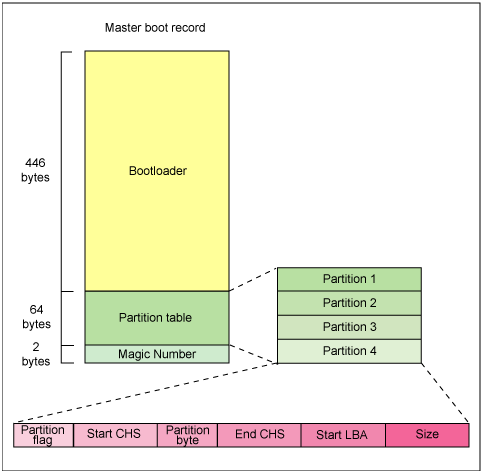
\includegraphics[width=.7\textwidth]{img/mbr}
  \caption{Структура MBR}
\end{figure}

Запись состоит из следующих полей:\\\\
\textbf{Bootloader}\\
Код начальной загрузки. Команды, используемые для определения местоположения и загрузки загрузочной записи раздела (VBR) с активного (загрузочного) раздела.\\\\
\textbf{Partition Table}\\
Главная таблица разделов. Таблица, состоящая из четырех 16-байтовых записей для четырех первичных логических разделов или трех первичных и одного расширенного разделов. Каждый первичный раздел определяет один логический диск, а расширенный раздел может быть разбит на несколько логических дисков. Каждая запись таблицы разделов имеет следующий формат:
\tabulinesep = 1mm
\begin{longtabu} to \textwidth {|X[1.2, c , m ] |X[c , m ] | X[2, c , m ]|}\firsthline\hline
\textbf{Смещение (байт)}&\textbf{Размер (байт)}&\textbf{Запись}\\ \hline \endfirsthead
0	&1&Boot Indicator\\ \hline
1-3	&3&Start CHS \\ \hline
4	&1&Partition-type\\ \hline
5-7	&3&End CHS\\ \hline
8-11&4&Starting Sector\\ \hline
12-15&4&Partition Size\\ \hline
\caption{Структура 16-байтной записи\cite{16byte}}
\end{longtabu}
\begin{enumerate}
\item \textbf{Boot Indicator}. Флаг типа раздела (активный, неактивный, некорректный и т.д.)
\item \textbf{Start CHS}. Адрес первого сектора раздела в формате CHS (Cylinder, Head, Sector). Представляет собой кортеж из трёх координат(цилиндр, головка, сектор). Цилиндр - совокупность дорожек (треков) заданного радиуса на всех пластинах (и всех сторонах пластин). Головка - номер считывающей головки (соответствует номеру пластины, с каждой поверхности считывает только одна головка). Сектор - градус угла поворота диска.
\item \textbf{Partition-type}. Тип файловой системы, расположенной на разделе. Например \textbf{0Bh} означает систему \textbf{FAT32}.
\item \textbf{End CHS}. Адрес последнего сектора раздела в формате CHS.
\item \textbf{Starting Sector}. Адрес первого сектора раздела в формате LBA (Logical Block Addressing). Формат аналогичен CHS, за исключением того что позволяет обращаться к разделам находящимся за пределами 7.8 ГБ и до 2.2 TB.
\item \textbf{Partition Size}. Число секторов раздела.
\end{enumerate}
\textbf{Примечание:} в текущий момент идет отказ от CHS в пользу LBA, причем размер LBA увеличили с 32 бит до 48, что позволяет работать с максимальной емкостью в 144 петабайта\cite{LBA}.\\\\
\textbf{Magic Number}\\
Двухбайтовая сигнатура \textbf{55AAh}, используемая для идентификации MBR.

\subsubsection{Вторичный загрузчик}
Вторичный загрузчик - программа расположенная в загрузочном секторе активного логического раздела \textbf{VBR}(Volume Boot Record).

Задачей вторичного загрузчика является поиск ядра в определенной файловой системе на разделе диска, загрузка ее в память и передача управления ядру ОС. Для этого вторичный загрузчик должен уметь работать с файловой системой, расположенной на данном разделе.

\tabulinesep = 1mm
\begin{longtabu} to \textwidth {|X[1.2, c , m ] |X[c , m ] | X[2, c , m ]|}\firsthline\hline
\textbf{Смещение (hex формат)}&\textbf{Размер (байт)}&\textbf{Запись}\\ \hline \endfirsthead
0	&3	&JMP на загрузчик\\ \hline
03	&8	&Название системы\\ \hline
0B	&25	&Блок параметров BIOS\\ \hline
24	&26	&Дополнительный блок параметров BIOS\\ \hline
3E	&448&Загрузчик\\ \hline
1FE	&2	&Сигнатура 55AAh\\ \hline
\caption{Структура VBR для ФС FAT}
\end{longtabu}
Итогом работы первичного и вторичного загрузчика является размещение ядра операционной системы в оперативной памяти, и далее, готовность к выполнению уже более высокоуровневых функций.

%\begin{figure}[H]
%  \centering
%  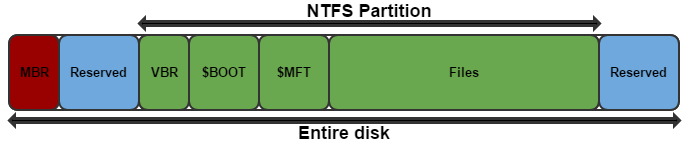
\includegraphics[width=\textwidth]{img/ntfs}
%  \caption{Структура NTFS}
%\end{figure}
%\subsubsection{Типы вторичных загрузчиков}
%
%\textbf{GRUB}

\subsection{Реализация простейшего первичного загрузчика}
Код первичного загрузчика приведен далее. Программа демонстрирует основную структуру первичного загрузчика и простейший принцип функционирования – в данном случае простой вывод приветственного сообщения.

Код основан на статье с хабрахабра\cite{mbrGuide} и приведен в приложении 1.
\subsubsection{Алгоритм программы}
Программа размещается при считывании в оперативной памяти начиная  с адреса 0x7C00h. Затем с использованием прерывания видео-сервиса BIOS 10h производится очищение экрана и установка видеорежима (сервис установки видеорежима; для возможности вывода цветного текста). После этого осуществляется циклический посимвольный вывод строки буфера, содержащей тестовое сообщение 
\subsubsection{Компиляция кода}
Для этого поставим yasm(\url{http://yasm.tortall.net/Download.html}) и выполним команду:
\begin{lstlisting}[language={}, caption={Компиляция ассемблерного кода}]
vsyasm.exe mbr.asm -f bin -o mbr
\end{lstlisting}
После этого был получен файл \textbf{mbr} размером в 512 байт. Дополнительно файлу было задано расширение \textbf{.iso}.
\subsubsection{Погдотовка виртуальной машины VMware}
Была создана пустая виртуальная машина. В её настройках была добавлен виртуальная дискета в которой был указан файл \textbf{mbr.iso}.
\begin{figure}[H]
  \centering
  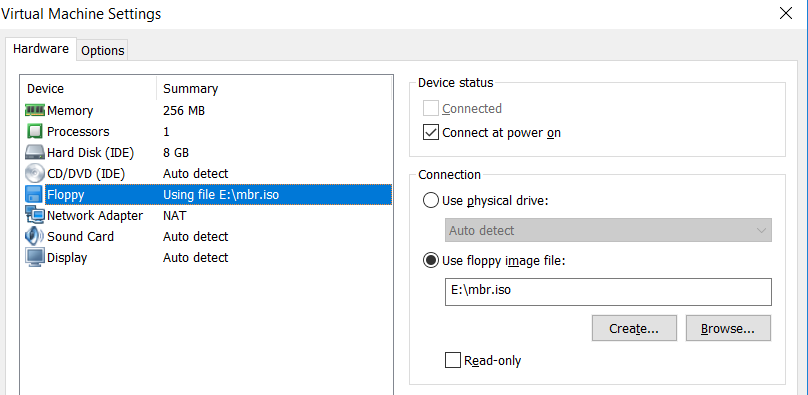
\includegraphics[width=.8\textwidth]{img/p1/4}
  \caption{Виртуальная дискета}
\end{figure}
\subsubsection{Тестирование}
Запускаем виртуальную машину. На экране появится надпись:
\begin{figure}[H]
  \centering
  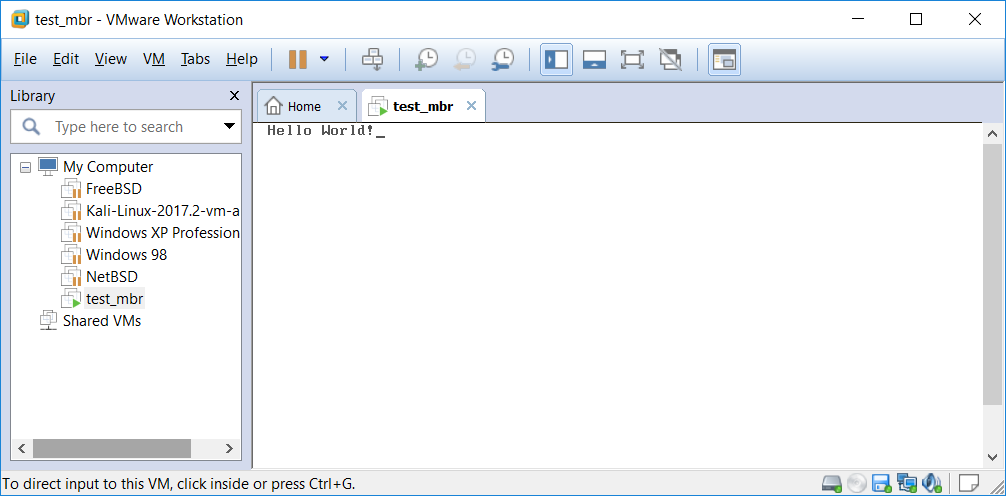
\includegraphics[width=.8\textwidth]{img/p1/5}
  \caption{Запуск первичного загрузчика}
\end{figure}
Как и ожидалось на экран вывелось приветственное сообщение. 

\subsection{Реализация на языке C}
На языке C, был реализован простейший первичный загрузчик.
\lstinputlisting[caption=mbr.c]{sourceCode/p1/c_realise/mbr.c}
Данный файл можно разделить на 3 области:
\begin{enumerate}
\item Область с различными \textbf{define}, где определяется размер сектора, адрес для загрузки, загружаемый сектор, а также некоторые макросы для используемых далее функций;
\item Функция \textbf{print}, которая печатает на экран некоторый текст, который был передан в данную функцию в качестве параметра;
\begin{itemize}
\item Реализация вывода аналогична прошлой, печать символов происходит до появления пустого символа.
\end{itemize}
\item Функция \textbf{main}, которая и вызвает функцию печати.
\end{enumerate}
Дополнительно, для удобства компиляции был создан \textbf{Makefile} с необходимыми клюами компиляции.
\lstinputlisting[caption=Makefile]{sourceCode/p1/c_realise/Makefile}

Для компиляции программы, необходимо выполнить команду \textbf{make}.

Тестирование будет произведено с использованием Qemu версии 2.5.0.

Выполним команду \textbf{qemu-system-x86\_64 boot.MBR}, после чего откроет окно QEMU:
\begin{figure}[H]
  \centering
  \fbox{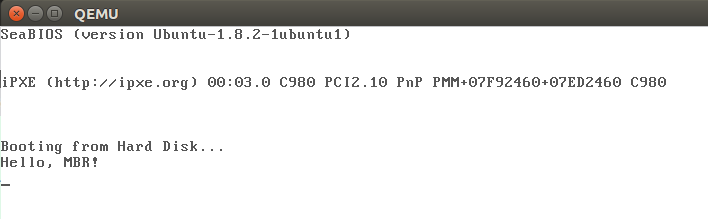
\includegraphics[width=.8\textwidth]{img/p1/QEMU}}
  \caption{Окно QEMU}
\end{figure}
Сообщение было успешно выведено.




\subsection{Реализация поиска и загрузки вторичного загрузчика}
В данной части работы проводится реализация первичного загрузчика, который находит необходимый файл на устройстве с определенной файловой системой. Также была выполнена реализация вторичного загрузчика, код которого загружается первичным загрузчиком для выполнения.

В качестве файловой системы выбрана FAT-12. Код загрузчиков основан на статье\cite{mbr2Guide} и приведен в приложении 2.

Первичный загрузчик осуществляет поиск файла с определенным заранее известным именем(bootor). Если первичный загрузчик находит его, то производит его загрузку в определенное место в оперативной памяти, после чего передает туда управление.

Вторичный загрузчик проверяет, что был загружен по определенному адресу, после чего выводит приветственное сообщение.

\subsubsection{Подготовка образа}
Для получения исполняемых файлов необходимо их скомпилировать:
\begin{lstlisting}[language={}, caption={Компиляция ассемблерного кода}]
vsyasm.exe bootor.asm -f bin -o BOOTOR
vsyasm.exe fat12.asm -f bin -o fat12
\end{lstlisting}
Далее с помощью программы \textbf{UltraISO} был создан образ \textbf{loader\_1.iso}  в корень которого был добавлен файл \textbf{BOOTOR}.
\begin{figure}[H]
  \centering
  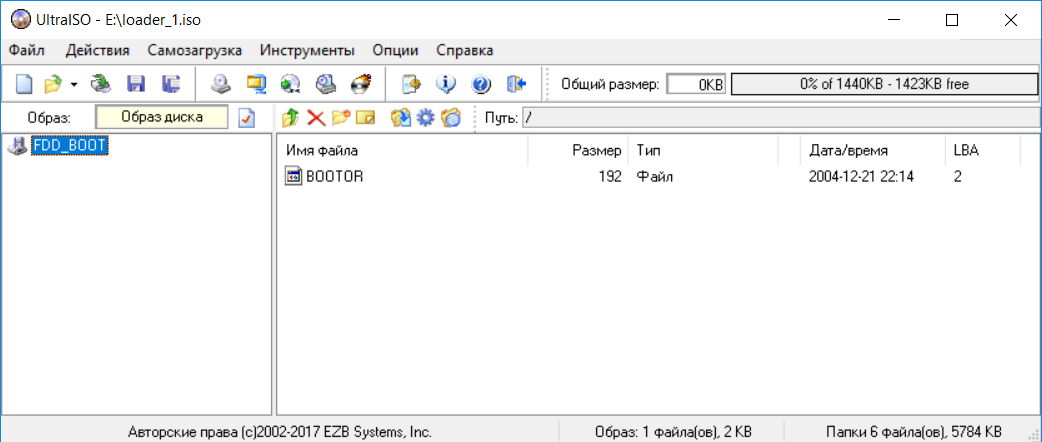
\includegraphics[width=\textwidth]{img/p2/1}
  \caption{Содержимое loader\_1.iso}
\end{figure}
Далее с помощью редактора \textbf{FlexHEX} был открыт бинарный код файлов \textbf{loader\_1.iso} и \textbf{fat12}.
\begin{figure}[H]
  \centering
  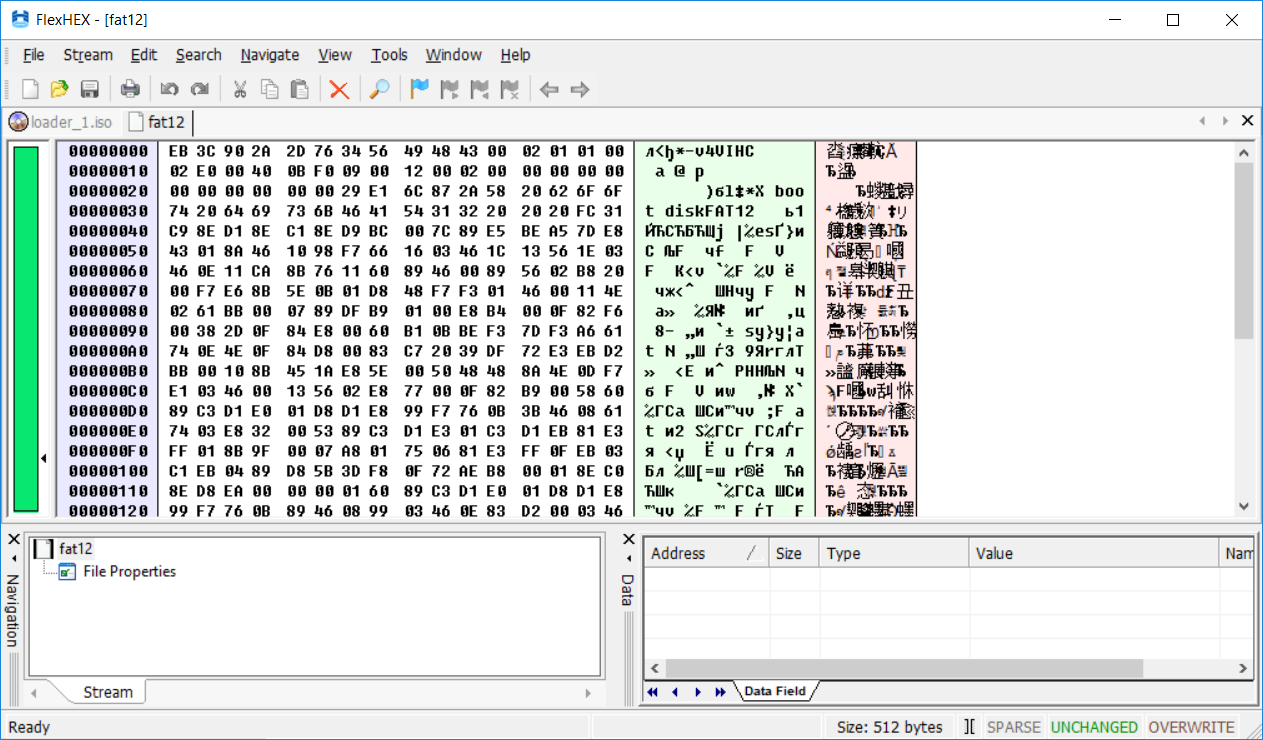
\includegraphics[width=\textwidth]{img/p2/2}
  \caption{Бинарный код fat12}
\end{figure}
В данном случае необходимо скопировать первые 512 байт(первый сектор) файла fat12 в начало файла loader\_1.iso.
\begin{figure}[H]
  \centering
  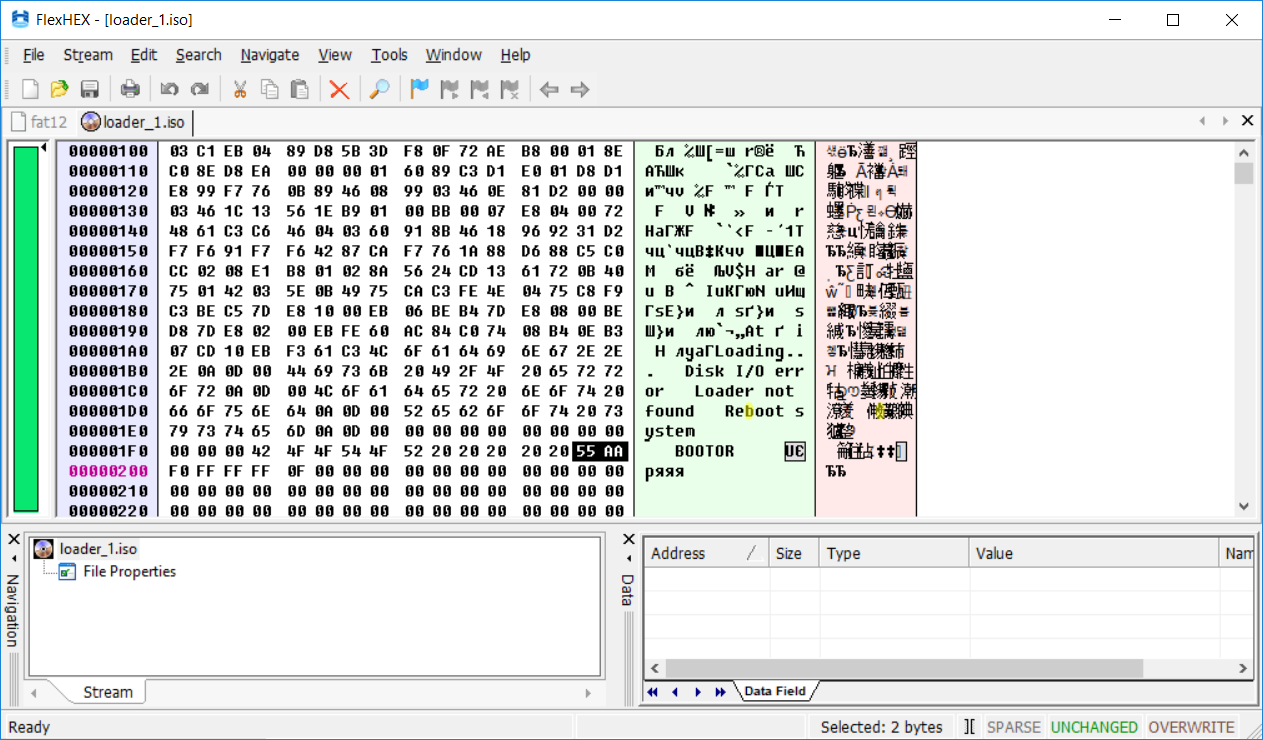
\includegraphics[width=\textwidth]{img/p2/3}
  \caption{Бинарный код loader\_1.iso}
\end{figure}
Последние два байта соответствуют сигнатуре \textbf{55AAh}.

Была создана пустая виртуальная машина, далее в её настройках был добавлен виртуальная дискета в которой был указан файл \textbf{loader\_1.iso}.
\begin{figure}[H]
  \centering
  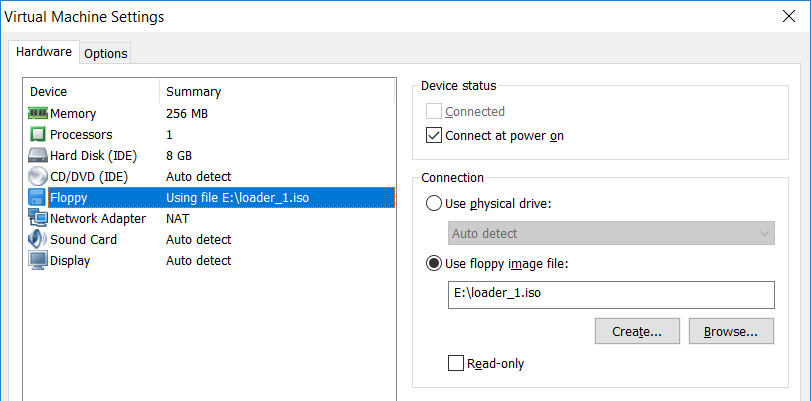
\includegraphics[width=.8\textwidth]{img/p2/4}
  \caption{Виртуальная дискета}
\end{figure}
Далее запускам виртуальную машину. В случае успеха было выведено приветственное сообщение вторичным загрузчиком.

\begin{figure}[H]
  \centering
  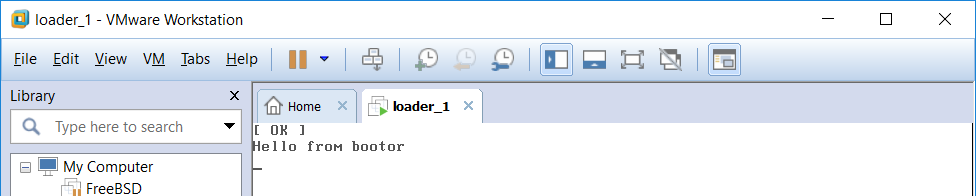
\includegraphics[width=\textwidth]{img/p2/6}
  \caption{Приветственное сообщение вторичного загрузчика}
\end{figure}
В случае, если например удалить файл bootor из образа, то будет выведено сообщение об ошибке.
\begin{figure}[H]
  \centering
  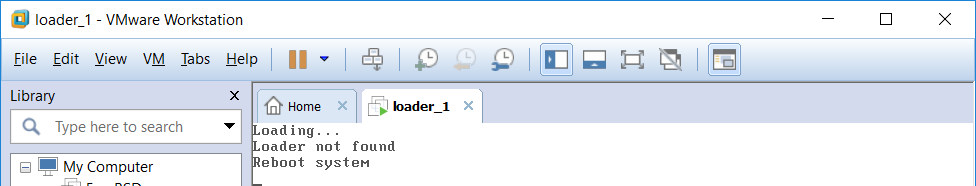
\includegraphics[width=\textwidth]{img/p2/5}
  \caption{Сообщение об ошибке}
\end{figure}
В результате работы удалось выполнить поиск определенного файла и передачи ему управления. Управление передавалось простейшему коду, который выводил приветственное сообщение. Но если производить поиск, загрузку и передачу управления не произвольному файлу, а ядру ОС, то будет произведена ее полноценная загрузка. 

%\subsection{Первичный загрузчик операционной системы MS-DOS}
%123

\subsection{Реализация мультизагрузчика}
Разметка MBR позволяет описать до 4 первичных разделов, каждый из которых может быть активным – то есть может содержать вторичный загрузчик. Также имеется возможность создать расширенный раздел, в котором можно описать ещё 4 раздела, но в данном случае, для упрощения расширенный раздел не анализируется.

Для загрузки, выступают следующие программы:
\begin{enumerate}
\item Ubuntu 16.04;
\item DrWeb livedisk 9.00;
\item Вывод на экран "мордочки".
\end{enumerate}
Алгоритм мультизагрузчика:
\begin{enumerate}
\item Для избежание проблемы того, что вторичный загрузчик будет скопирован на место первичного загрузчика, необходимо заранее скопировать первичный загрузчик с адреса \textbf{7C00h} в безопасную область памяти, в данном случае, безопасной областью выбран адрес \textbf{60h};
\item Поиск активных разделов и вывод их номеров, для этого анализируются все четыре записи таблицы разделов, на предмет наличия записи активного раздела - 80h;
\item Ожидание ввода номера раздела с клавиатуры. Для чтения нажатой клавиши используется прерывание BIOS \textbf{int 16h}, после чего производится сравнение ASCII кода введенной клавиши с номерами активных разделов;
\item Загрузка первого сектора(вторичного загрузчика) выбранного активного раздела по адресу 7C00h  и передача управления по этому адресу. Загрузка первого сектора производится с помощью прерывания BIOS \textbf{int 13h}.
\end{enumerate}
Исходный код мультизагрузчика, приведен в приложении 3, в листинге \ref{p3:MultiBoot}.

\subsubsection{Подготовка накопителя}
Работа будет производится на реальном устройстве - USB флэшке емкостью 32 Гб. Средствами, встроенной в Windows утилиты - \textbf{управление дисками}, устройство было размечено следующим образом:
\begin{figure}[H]
  \centering
  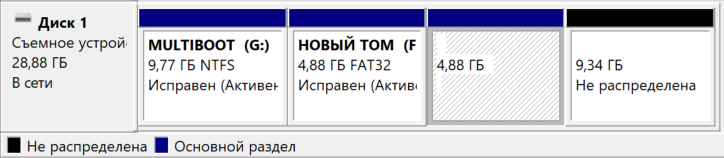
\includegraphics[width=\textwidth]{img/p3/usbArch}
  \caption{Разметка носителя}
\end{figure}
Где:
\begin{itemize}
\item Первый раздел(G) с ФС \textbf{NTFS} - для Ubuntu;
\item Второй раздел(F) с ФС \textbf{FAT32} - для DrWeb;
\item Третий раздел, без ФС - для "мордочки".
\end{itemize}

\subsubsection{Запись Ubuntu 16.04}
Основная проблема с корректностью запуска ОС, связана с корректностью записи на носитель программы загрузчика. Например, при записи DrWeb livedisk, никаких проблем не возникло, так как программа и предназначалась для подобных целей. То в данном случае, столкнулся со следующими проблемами:
\begin{itemize}
\item Большинство программ для записи были не в состоянии записать образ на конкретный раздел, большинство из них предлагало перезаписать в USB-накопитель.
\item Оставшиеся программы, некорректно записывали ОС, в следствии чего, вторичный загрузчик сообщал о том что не может найти необходимые файлы.
\end{itemize}
Путем проб и ошибок, выбор пал на программу \textbf{YUMI – Multiboot USB Creator}, которая использует в виде вторичного загрузчика - модифицированный загрузчик syslinux.
\begin{figure}[H]
  \centering
  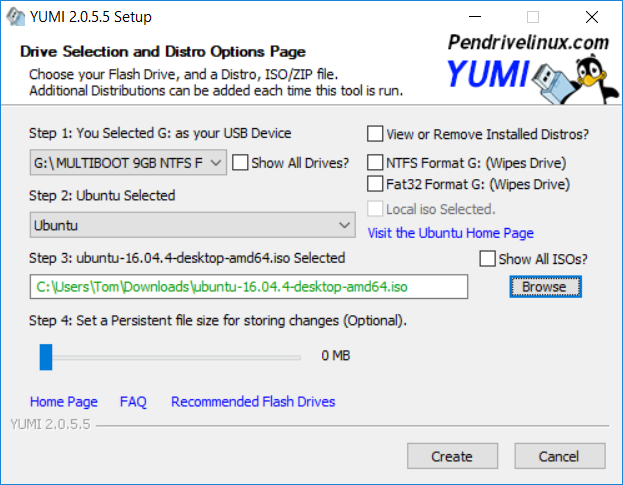
\includegraphics[width=.9\textwidth]{img/p3/yumi}
  \caption{Подготовка к записи ОС, с использованием Yumi}
\end{figure}


\subsubsection{Запись DrWeb LiveDisk 9.00}
\begin{figure}[H]
  \centering
  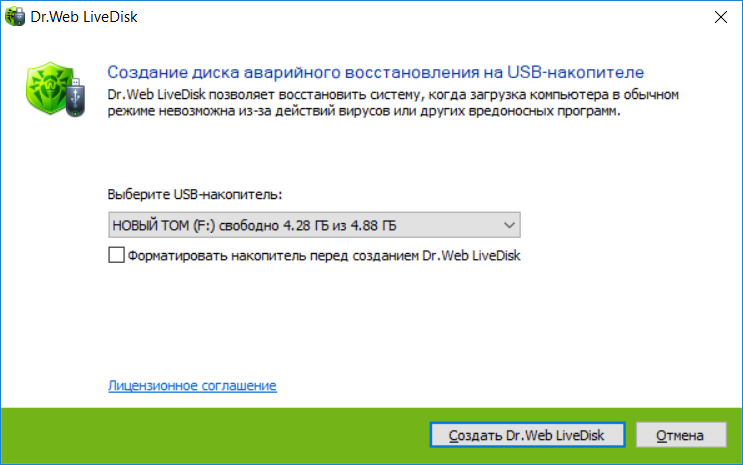
\includegraphics[width=.8\textwidth]{img/p3/drweb}
  \caption{Запись DrWeb}
\end{figure}
После записи, раздел на который была произведена установка станет активным.

\subsubsection{Запись мордочки}
В качестве "мордочки$"$, будет выступать следующие изображение:
\begin{figure}[H]
  \centering
  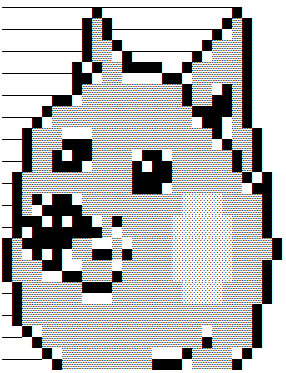
\includegraphics[width=.35\textwidth]{img/p3/doge}
  \caption{"Мордочка"}
\end{figure}
Программа, для вывода "мордочки" расположена в приложении 3, листинге \ref{p3:doge}, где каждый выводимый символ задан в виде ASCII кода символа.

Для получения ASCII кодов символов, на языке \textbf{Python} был написан специальный конвертер, который представлен в приложении 3, листинге \ref{p3:readFile}.

Алгоритм которого заключается в посимвольно чтении исходного файла с изображением, где для каждого символа, используя словарь(символ - код) выводится его код.

После компиляции ассемберного кода, с помощью редактора \textbf{HxD} открываем его, а также 0 сектор USB-накопителя.
\begin{figure}[H]
  \centering
  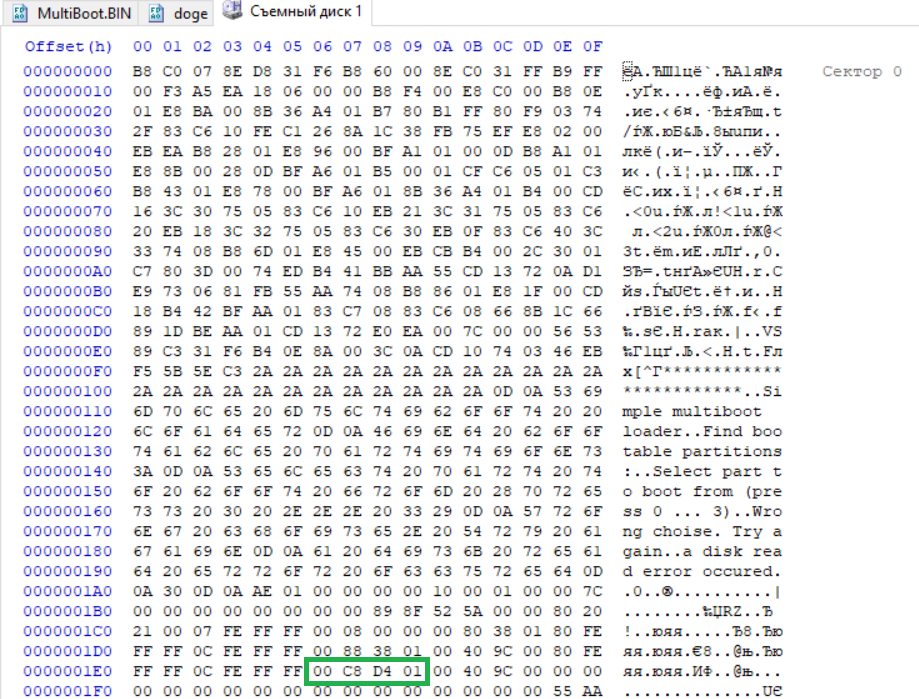
\includegraphics[width=.9\textwidth]{img/p3/third}
  \caption{0 сектор USB-накопителя}
\end{figure}
Зеленой рамкой выделен адрес, по которому начинается данный раздел. В данном случае это \textbf{01 D4 C8 00}(адрес читается задом наперед).

Если открыть калькулято в режиме программиста и ввести данный адрес, то его \textbf{DEC} значение будет означать номер сектора.
\begin{figure}[H]
  \centering
  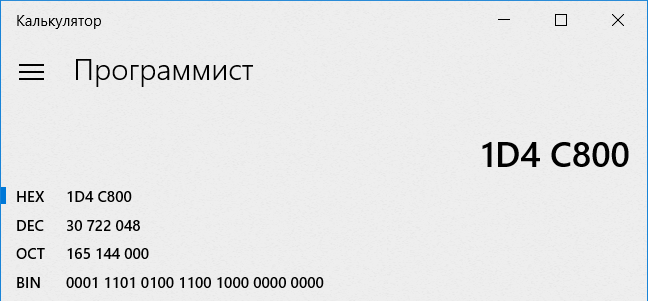
\includegraphics[width=.7\textwidth]{img/p3/calc}
  \caption{Определение сектора}
\end{figure}
Перейдем по данному сектору, и скопируем в него данные из скомпилированный программы по выводу "мордочки".

Конечный результат, должен выглядеть следующим образом:
\begin{figure}[H]
  \centering
  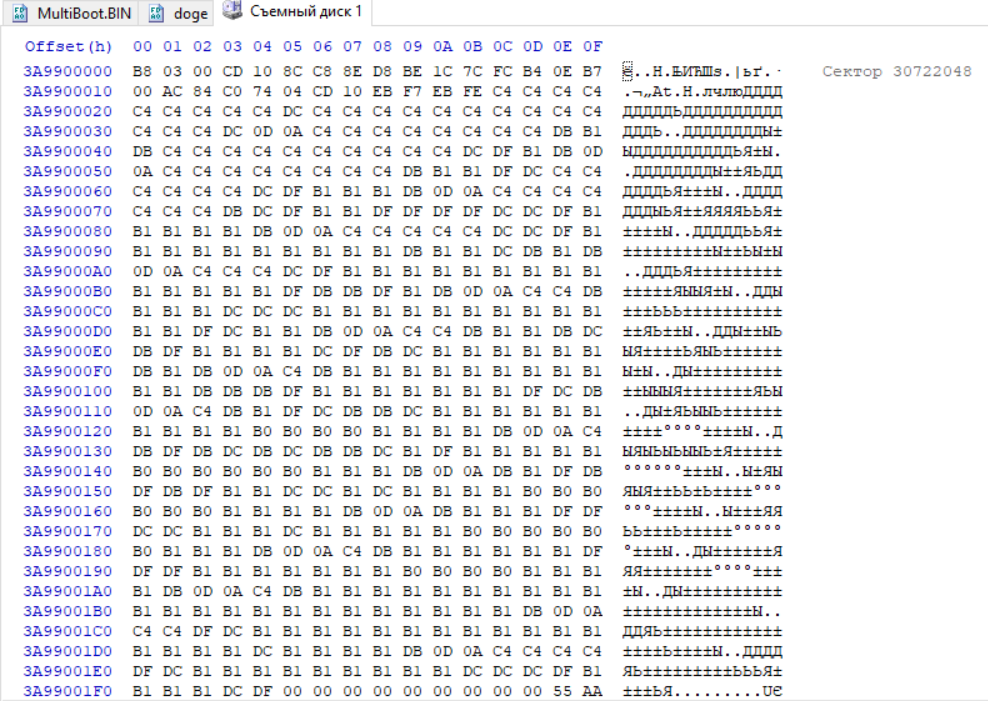
\includegraphics[width=.9\textwidth]{img/p3/thirdDoge}
  \caption{0 сектор третьего раздела}
\end{figure}

\subsubsection{Модификация первичного загрузчика}
Теперь необходимо заменить код в 0 секторе, на код мультизагрузчика, итоговый результат должен выглядеть следующим образом:
\begin{figure}[H]
  \centering
  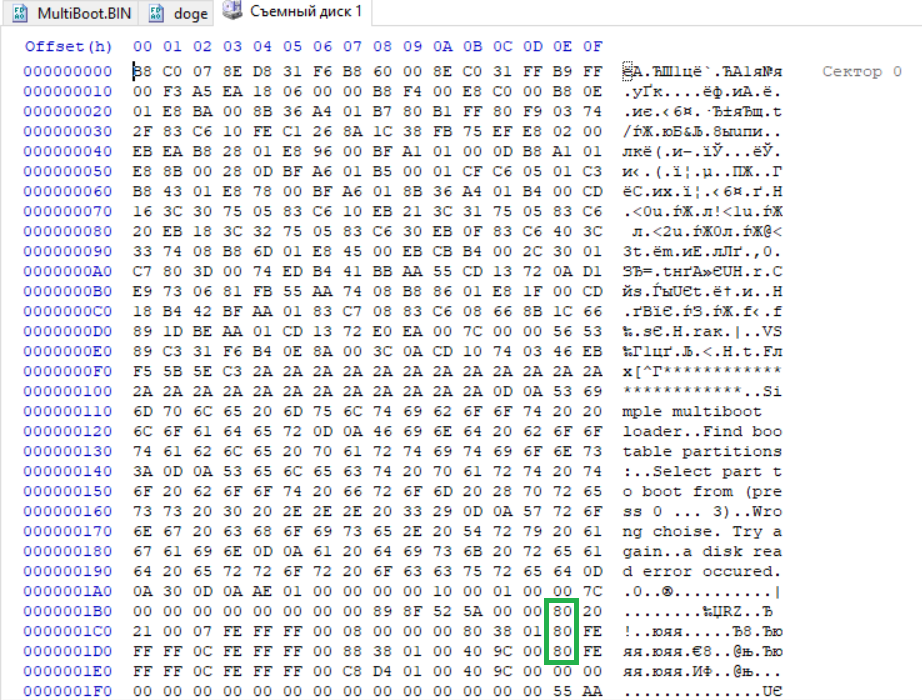
\includegraphics[width=.9\textwidth]{img/p3/actives}
  \caption{0 сектор USB-накопителя}
\end{figure}
Зеленой рамкой выделены индикаторы активных разделов, в данном случае необходимо выставить значение \textbf{80h}.

\subsubsection{Тестирование}
После подключения USB - накопителя к компьютеру, необходимо зайти в меню выбора устройства, с которого необходимо произвести загрузку.
\begin{figure}[H]
  \centering
  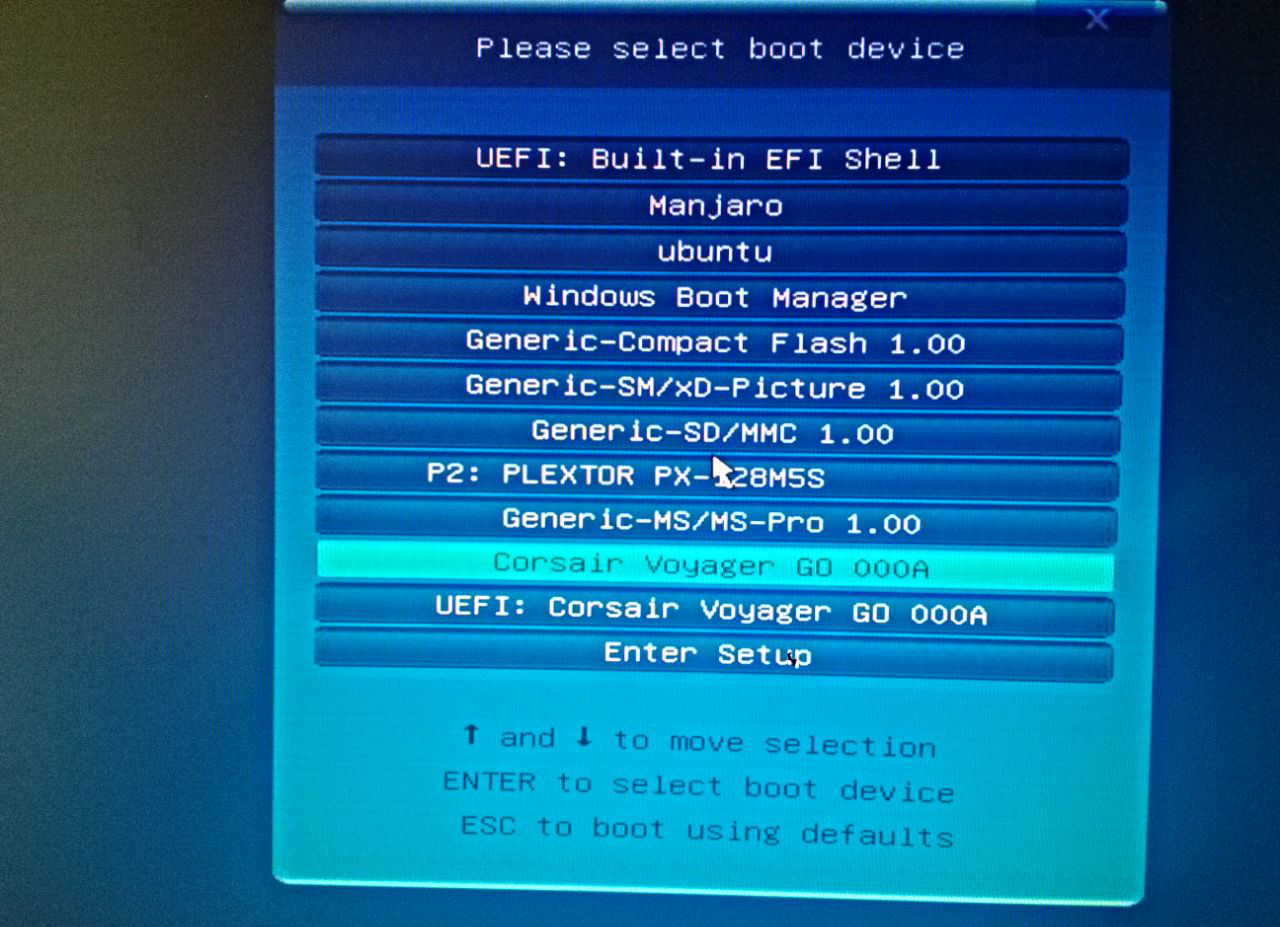
\includegraphics[width=.8\textwidth]{img/p3/testing/1}
  \caption{Выбор устройства для загрузки}
\end{figure}
В данном случае это \textbf{Corsair Voyager GO 000A}.

Далее следует меню мультизагрузчика, который успешно определил три активных сектора.
\begin{figure}[H]
  \centering
  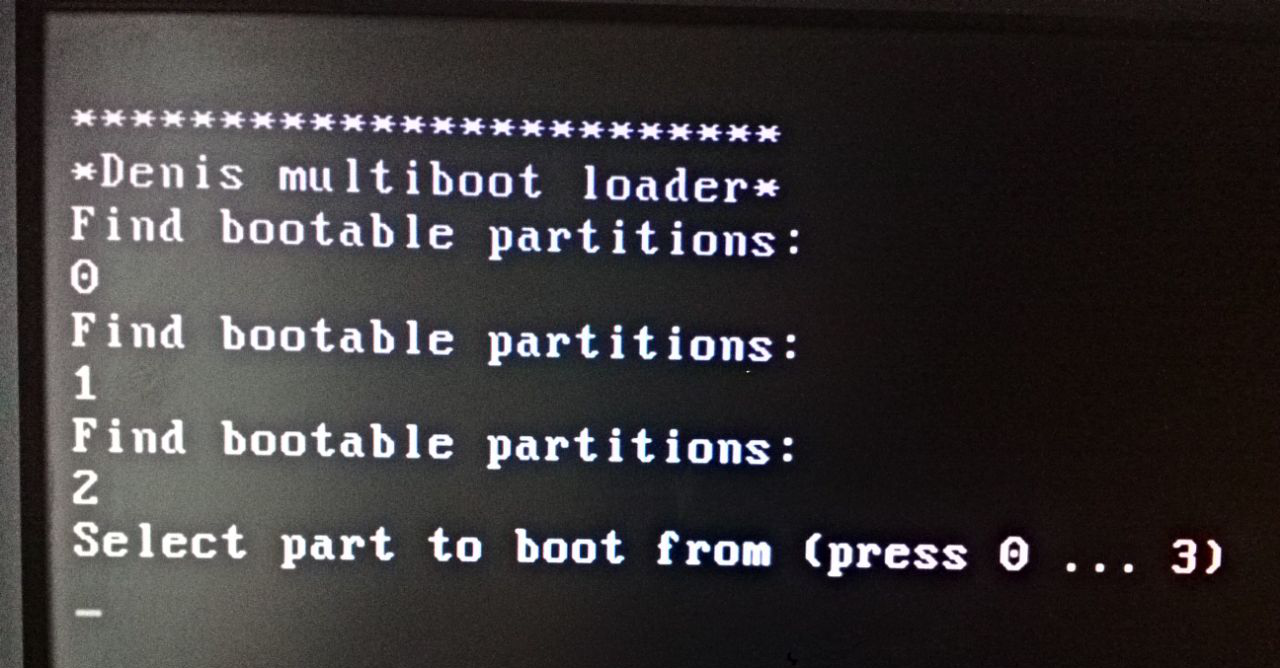
\includegraphics[width=.8\textwidth]{img/p3/testing/2}
  \caption{Меню мультизагрузчика}
\end{figure}
Выберем 0 раздел, после чего будет загружен вторичный загрузчик Yumi.
\begin{figure}[H]
  \centering
  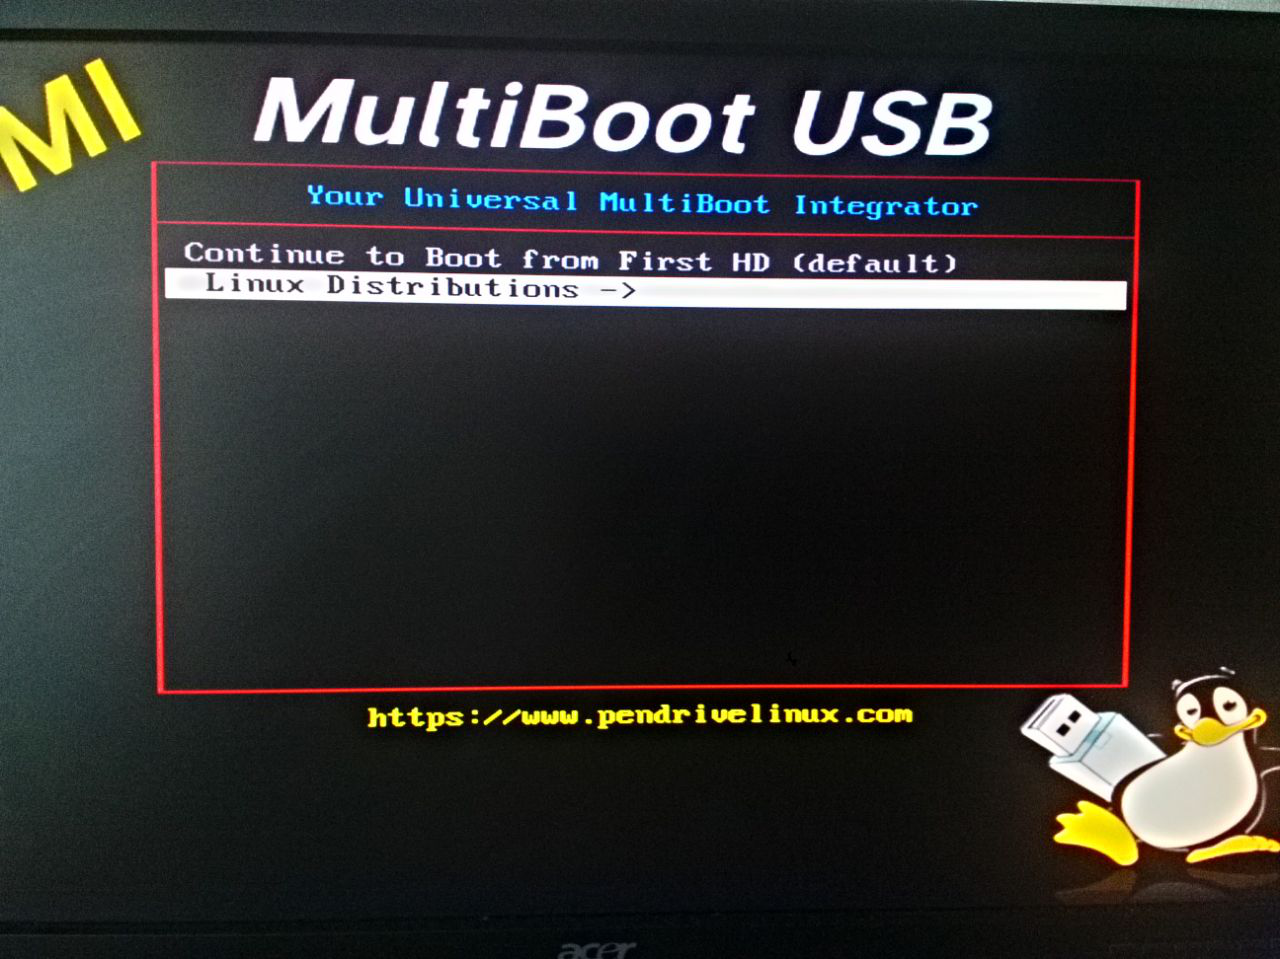
\includegraphics[width=.8\textwidth]{img/p3/testing/3}
  \caption{Меню Yumi}
\end{figure}
Выберем пункт \textbf{Linux Distributions}, после чего будет открыто окно выбора ОС.
\begin{figure}[H]
  \centering
  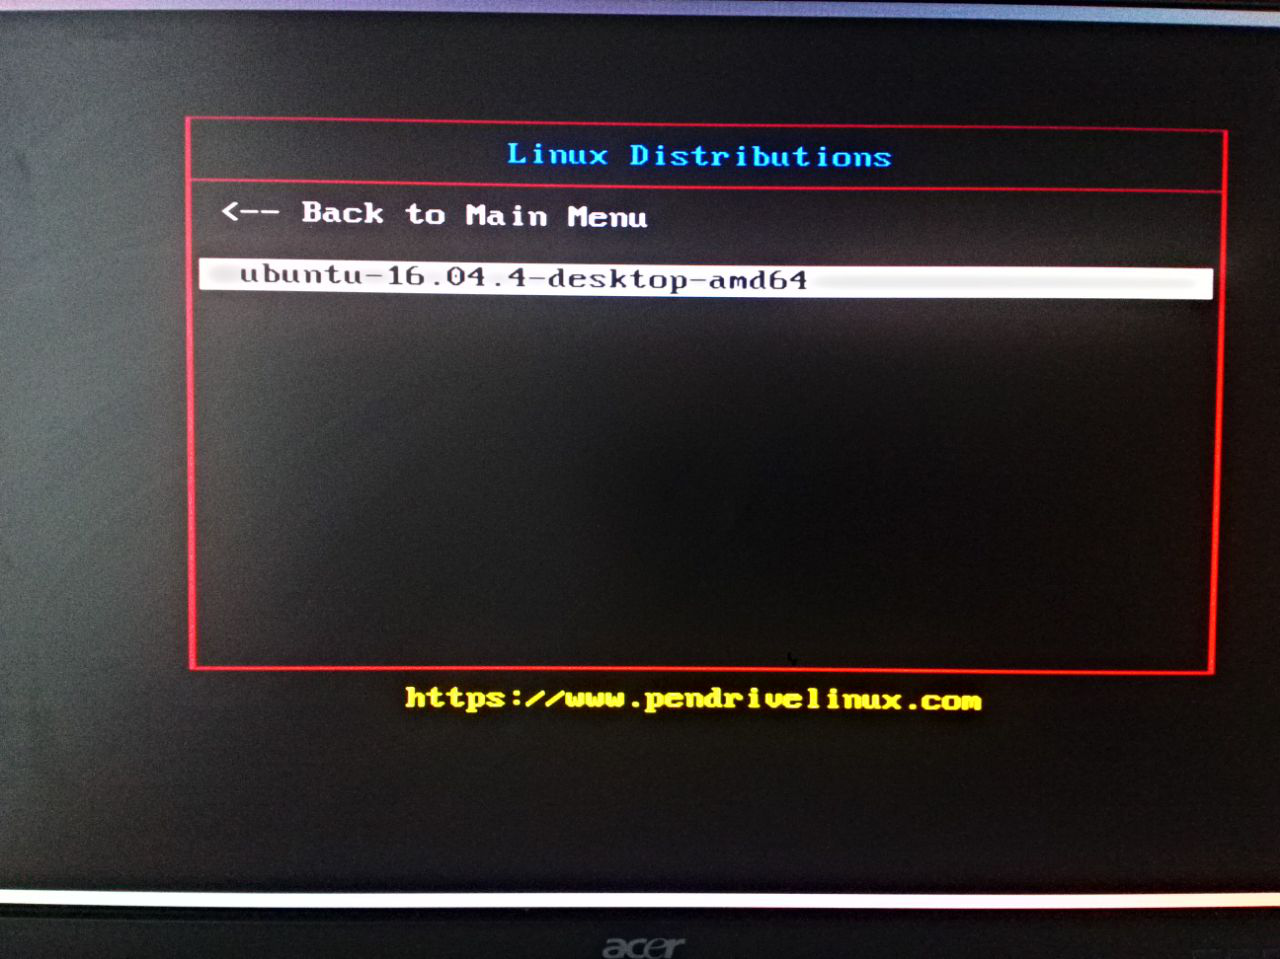
\includegraphics[width=.8\textwidth]{img/p3/testing/4}
  \caption{Меню выбора ОС}
\end{figure}
При выборе Ubuntu, начнется загрузка ОС.

Если выбрать 1 раздел, то будет загружен DrWeb.
\begin{figure}[H]
  \centering
  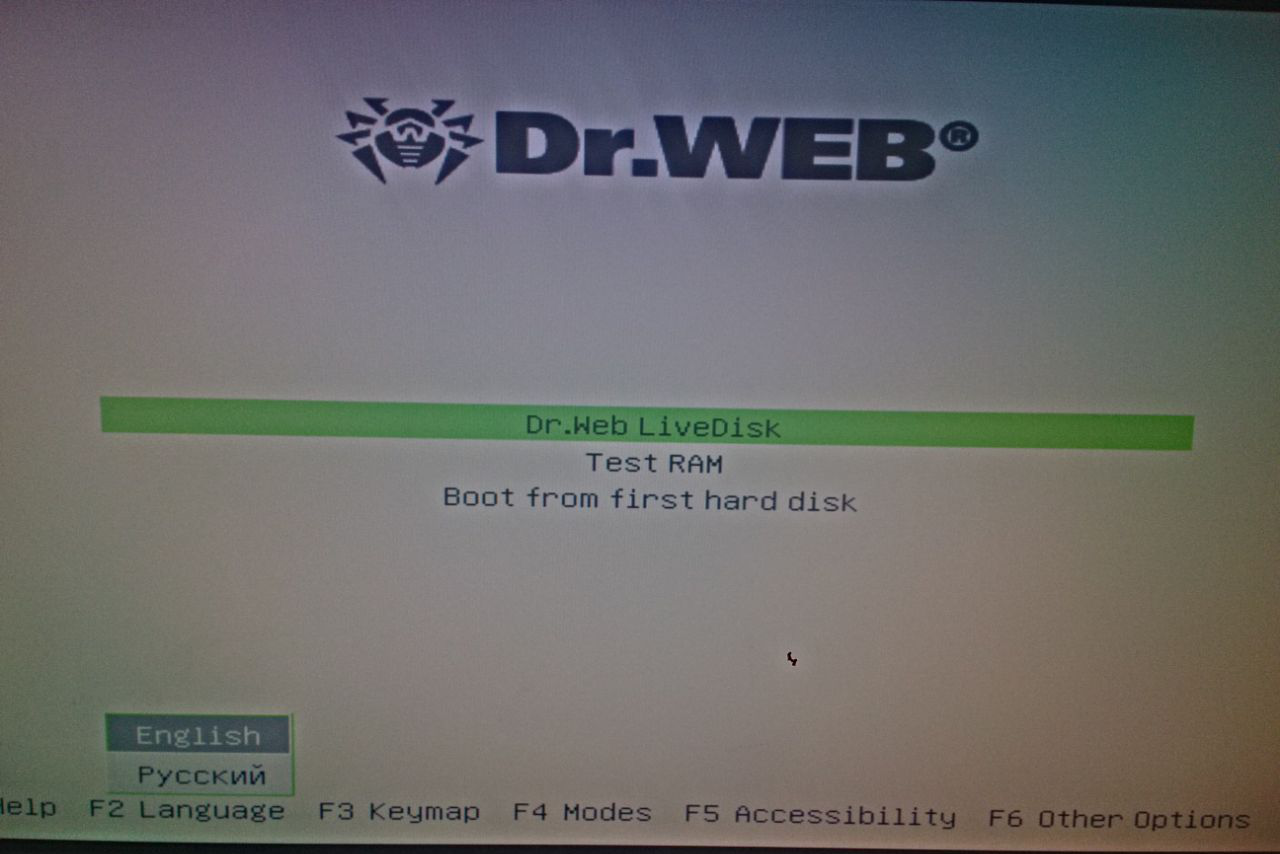
\includegraphics[width=.8\textwidth]{img/p3/testing/5}
  \caption{Приветственный экран DrWeb}
\end{figure}

И наконец, если выбрать 2 раздел, то будет выведена "мордочка".
\begin{figure}[H]
  \centering
  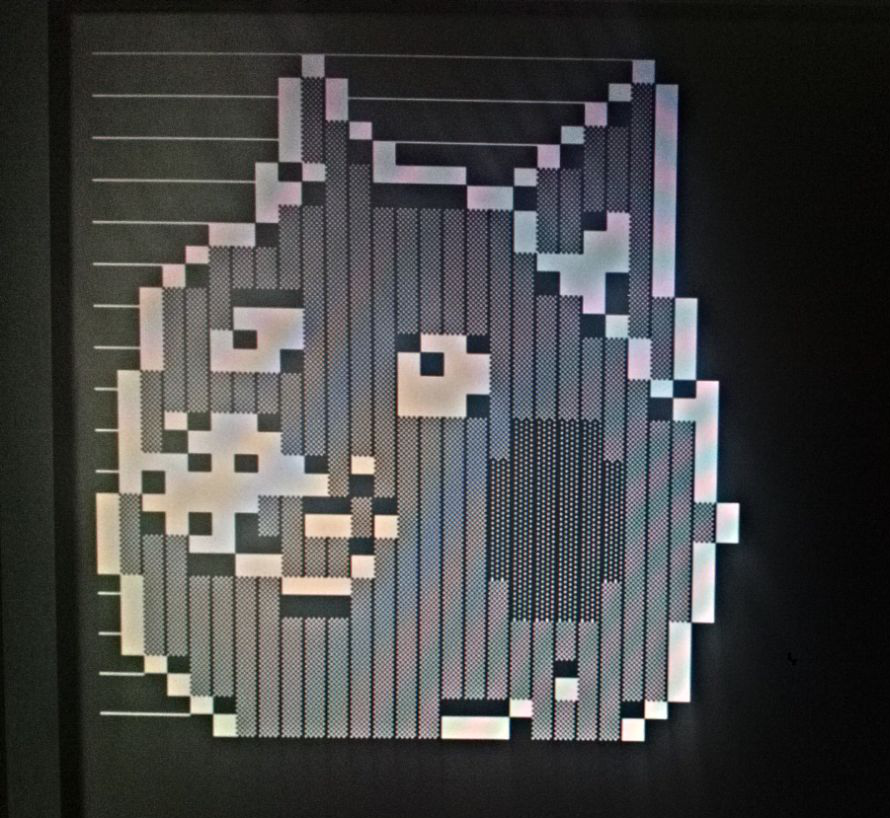
\includegraphics[width=.6\textwidth]{img/p3/testing/6}
  \caption{"Мордочка"}
\end{figure}



\subsection{Первичный загрузчик ОС}
\subsubsection{Алгоритм работы}
В качестве ОС выступает ms dos версии 6.22, сам первичный загрузчик написан на основе кода из гитхаба\cite{github} в котором был дизассемблирован загрузчик DOS.

Алгоритм работы:
\begin{enumerate}
\item Копирование таблицы параметров дискеты (DPT), на которую указывает вектор прерывания 1E;
\item Изменение копии DPT;
\item Изменение вектора прерывания, чтобы он указывал на измененную копию DPT;
\item Сброс контроллера дискеты – с помощью прерывания int 13;
\item Вычисление адреса корневого каталога дискеты;
\item Чтение первого секторы корневого каталога по адресу 0000:0500h;
\item Проверка, что первые два элемента в корневом каталоге – это файлы IO.SYS и MSDOS.SYS;
\item Чтение первых трех секторов IO.SYS по адресу 0070:0000h;
\item Передача управления на адрес 700h.
\end{enumerate}

Исходный код приведен в приложении 4, листинге \ref{p4:dosBoot}.

\subsubsection{Подготовка}
При создании загрузочной дискеты, необходимо корректно записать записать файлы операционной системы. В частности первыми файлами в корневой директории должны быть \textbf{IO.SYS} и \textbf{MSDOS.SYS}, в противном случае система не загрузится.

На рисунке далее, приведена корневая директория уже подготовленной дискеты:
\begin{figure}[H]
  \centering
  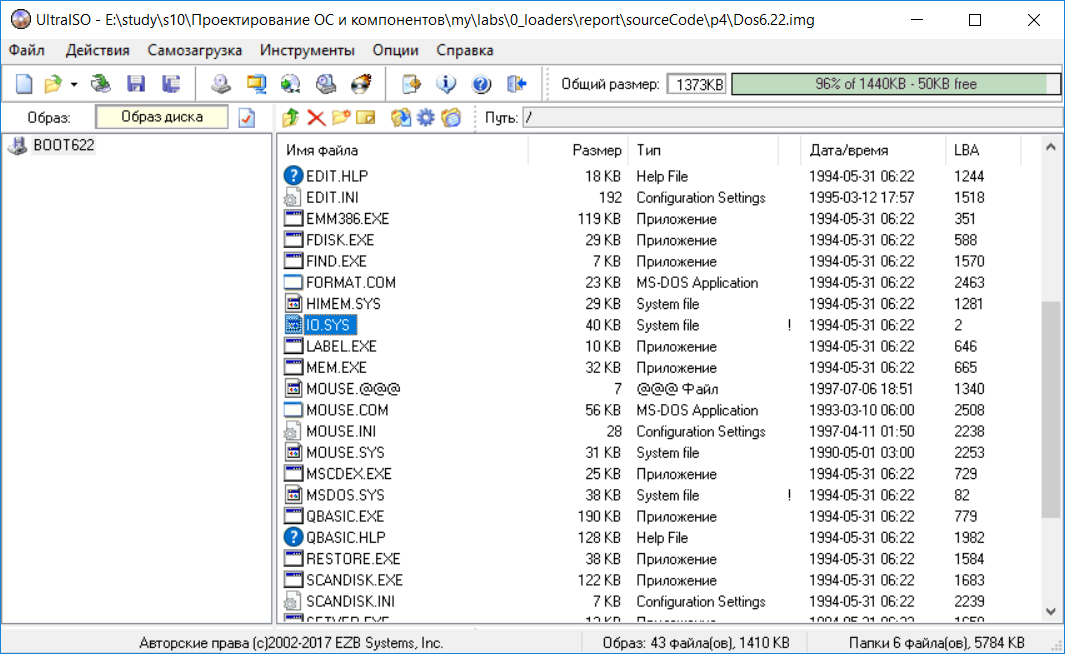
\includegraphics[width=\textwidth]{img/p4/1}
  \caption{Корень дискеты}
\end{figure}
После создания образа дискеты, в загрузочный сектор с помощь редактора \textbf{HxD} был занесен код загрузчика:
\begin{figure}[H]
  \centering
  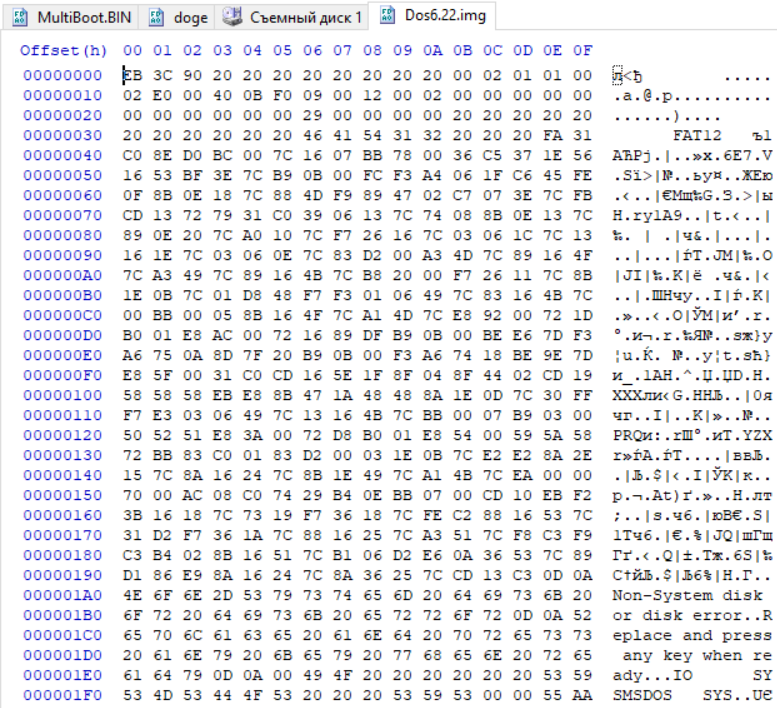
\includegraphics[width=.8\textwidth]{img/p4/2}
  \caption{Загрузочный сектор дискеты}
\end{figure}
\subsubsection{Тестирование}
Для тестирования была создана виртуальная машина, в настройках которой была добавлена виртуальная дискета, в которой был указан файл дискеты - \textbf{Dos6.22.img}. 
\begin{figure}[H]
  \centering
  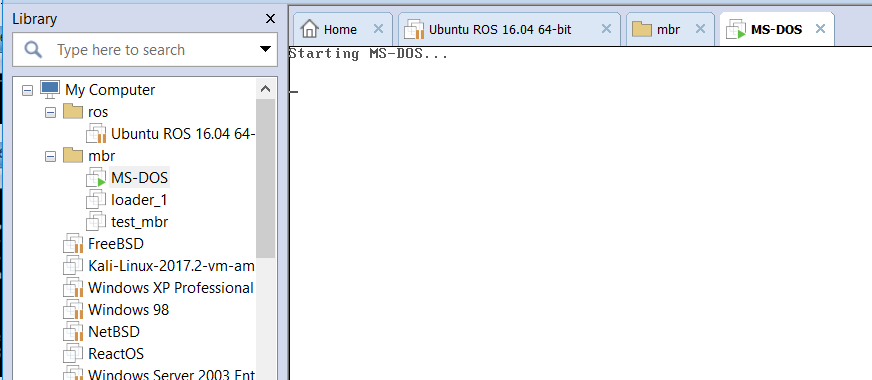
\includegraphics[width=\textwidth]{img/p4/3}
  \caption{Сообщение о загрузке MsDOS}
\end{figure}
\begin{figure}[H]
  \centering
  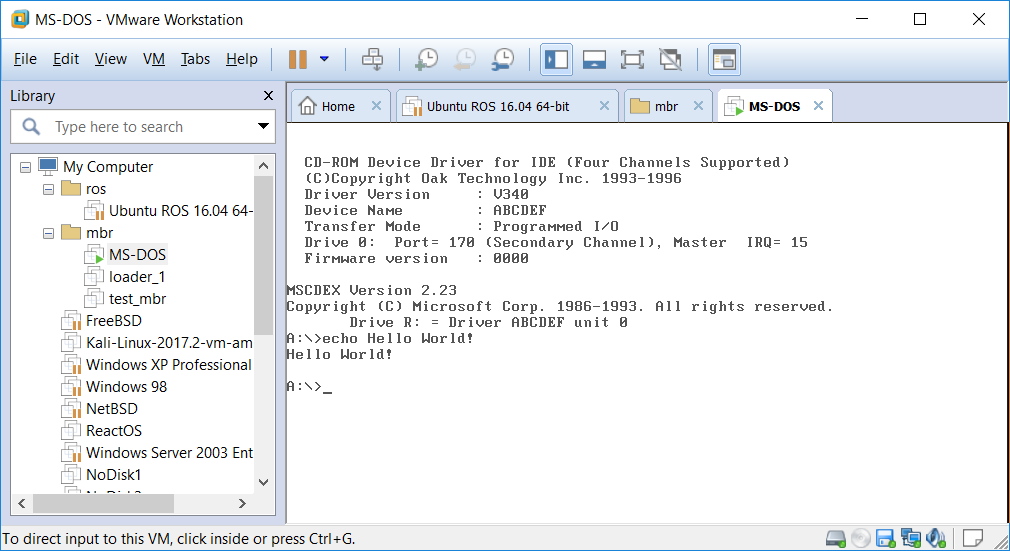
\includegraphics[width=\textwidth]{img/p4/4}
  \caption{Загруженная MsDOS}
\end{figure}
Образ дискеты также прикреплен к отчету.




\clearpage
\section*{Вывод}
\addcontentsline{toc}{section}{Вывод}
В данной работе были анализированы первичный и вторичный загрузчики, которые впоследствии были реализованы, в том числе при реализации мультизагрузчика.

При реализации мультизагрузчика, корректная запись загружаемой программы, как оказалось, не такая простоя задача. Дело в том, что вторичный загрузчик этих программ записывается некорректным образом. Для решения этой проблемы используются специализированные программы, но большинство из них неспособны записать программу(операционную систему) на какой-либо конкретный раздел накопителя, вместо этого предлагается лишь один раздел.

Подобная проблема также возникла при создании образа \textbf{MS-DOS}, где необходимо было разместить, файлы для загрузки системы, в определенной последовательности.

Реализованные в данной работе программы, демонстрирует основные принципы функционирования загрузчиков ОС, а также мультизагрузчиков, которые позволяют иметь несколько ОС на одном носителе.


%------------------------------------------------------------------------------

\nocite{github2}

\clearpage
\addcontentsline{toc}{section}{Список литературы}
\bibliography{thesis}
\bibliographystyle{ugost2008}

\clearpage
\addcontentsline{toc}{section}{Приложения}
\setcounter{section}{0}
\section*{Приложение 1} \label{p1:1}
\textbf{Простейший первичный загрузчик}
\lstinputlisting[caption=mbr.asm, label={p1:mbr}]{sourceCode/p1/mbr.asm}

\section*{Приложение 2} \label{p2:1}
\textbf{Первичный загрузчик для устройства с файловой системой FAT-12}
\lstinputlisting[caption=fat12.asm, label={p2:fat12}]{sourceCode/p2/fat12.asm}

\textbf{Вторичный загрузчик}
\lstinputlisting[caption=bootor.asm, label={p2:bootor}]{sourceCode/p2/bootor.asm}

\section*{Приложение 3} \label{p3:1}
\textbf{Программа по выводу "мордочки" на экран}
\lstinputlisting[caption=doge.asm, label={p3:doge}]{sourceCode/p3/doge.asm}

\textbf{Алгоритм по преобразованию ascii символов в их код}
\lstinputlisting[caption=readFile.py, label={p3:readFile}, language={[x86masm]Assembler}]{sourceCode/ascii/readFile.py}
К сожалению, в отчет не удалось прикрепить файл, где расположена "мордочка" для вывода на дисплей, из-за невозможности отображения дополнительных символов ascii, что так-же можно заметить в листинге выше.\\\\

\textbf{Мультизагрузчик}
\lstinputlisting[caption=MultiBoot.ASM, label={p3:MultiBoot}]{sourceCode/p3/MultiBoot.ASM}

\section*{Приложение 4} \label{p4:1}
\textbf{Первичный загрузчик ОС}
\lstinputlisting[caption=dosBoot.asm, label={p4:dosBoot}]{sourceCode/p4/dosBoot.asm}


\end{document}